%master_report.tex, can't be edited - Mark
% edit the content.tex file instead
\documentclass[a4paper,11pt,hidelinks]{report}
\usepackage[utf8]{inputenc}
\usepackage{amsmath}
\usepackage[titletoc,toc,page]{appendix}

\usepackage[english]{babel}
\usepackage{graphicx}
\usepackage{subcaption}
\usepackage{amssymb}
\usepackage{titlesec}
\usepackage{helvet}
\renewcommand{\familydefault}{\sfdefault}
\usepackage{calc}
\usepackage{amsfonts}
\usepackage{lipsum}
\usepackage[amsmath,amsthm,thmmarks]{ntheorem}
\usepackage{fancyvrb}
\usepackage{setspace}
\usepackage[T1]{fontenc}
\doublespacing
\usepackage{url}
\usepackage{letltxmacro}
%\usepackage{bigints}
\usepackage{soul}
\usepackage[top=20mm,left=20mm,right=20mm,bottom=20mm,footskip=25pt]{geometry} %was 0.14in, don't know why - Mark
\usepackage{fancyhdr}
\usepackage{footnote}
\usepackage{appendix}
\usepackage{siunitx}
\usepackage{multirow}
\usepackage{wrapfig}
\usepackage{textgreek}
\usepackage{longtable}
\usepackage{bigstrut}
\usepackage[table,dvipsnames]{xcolor}
\usepackage{pdfpages}
\usepackage{titling}
\usepackage{csquotes}
\usepackage{pbox}
\usepackage{booktabs}
\usepackage[export]{adjustbox}
\usepackage{array}
\newcolumntype{C}[1]{>{\centering\arraybackslash}p{#1}}
%\usepackage{pbox}
\usepackage{rotating}   % added by Mark for use in table
\usepackage{pifont}     % added by Mark to include tick symbols in table
\usepackage{listings}   % added by Xiaonan to include Matlab code
\lstset{
basicstyle=\small\ttfamily,
columns=flexible,
breaklines=true
}
\usepackage{caption}    % changed to caption / should still work
\usepackage{tocloft}    % added by Mark for TOC names
\usepackage{textcomp}
\setcounter{tocdepth}{4}
\setcounter{secnumdepth}{4}

%References & bibliography - add your own .bib files with \addbibresource command
\usepackage[backend=bibtex,style=numeric-comp,sorting=none]{biblatex}   % Disabled Sorting - Mark
\DeclareBibliographyAlias{webpage}{online}  %ignore warnings
\bibliography{bib}

\AtBeginDocument{\let\latexlabel\label}

\titleformat{\chapter}[hang]
{\normalfont\huge\bfseries}{\thechapter}{17.5pt}{\huge}
\titlespacing*{\chapter}{0pt}{-40pt}{0pt}
\titlespacing*{\section}{0pt}{0pt}{0pt}
\titlespacing*{\subsection}{0pt}{0pt}{0pt}
\titlespacing*{\subsubsection}{0pt}{0pt}{0pt}   %reduce spacing to fit with other stuff


%Remove the Page number from the part pages - Mark
\makeatletter
\renewcommand\part{%
    \if@openright
    \cleardoublepage
    \else
    \clearpage
    \fi
    \thispagestyle{empty}%   % Original »plain« replaced by »emptyx
    \addtocounter{page}{-1} %Decrease the page counter so the part page doesn't count, added by Mark
    \if@twocolumn
    \onecolumn
    \@tempswatrue
    \else
    \@tempswafalse
    \fi
    \null\vfil
    \secdef\@part\@spart}
\makeatother
% From http://tex.stackexchange.com/questions/54115/how-to-let-part-stay-solo-page-and-no-page-number


\newcommand\numberthis{\addtocounter{equation}{1}\tag{\theequation}}
% All sqrts closed
\LetLtxMacro{\oldsqrt}{\sqrt}
\renewcommand{\sqrt}[1][]{%
    \def\DHLindex{#1}\mathpalette\DHLhksqrt}
\def\DHLhksqrt#1#2{%
    \setbox0=\hbox{$#1\oldsqrt[\DHLindex]{#2\,}$}\dimen0=\ht0
    \advance\dimen0-0.2\ht0
    \setbox2=\hbox{\vrule height\ht0 depth -\dimen0}%
    {\box0\lower0.71pt\box2}}

\makeatletter
\newcommand*\@dblLabelI {}
\newcommand*\@dblLabelII {}
\newcommand*\@dblequationAux {}

\def\@dblequationAux #1,#2,%
{\def\@dblLabelI{\label{#1}}\def\@dblLabelII{\label{#2}}}

\newcommand*{\doubleequation}[3][]{%
    \par\vskip\abovedisplayskip\noindent
    \if\relax\detokenize{#1}\relax
    \let\@dblLabelI\@empty
    \let\@dblLabelII\@empty
    \else % we assume here that the optional argument
    % has the required shape A,B
    \@dblequationAux #1,%
    \fi
    \makebox[0.5\linewidth-1.5em]{%
        \hspace{\stretch2}%
        \makebox[0pt]{$\displaystyle #2$}%
        \hspace{\stretch1}%
    }%
    \makebox[0.5\linewidth-1.5em]{%
        \hspace{\stretch1}%
        \makebox[0pt]{$\displaystyle #3$}%
        \hspace{\stretch2}%
    }%
    \makebox[3em][r]{(%
        \refstepcounter{equation}\theequation\@dblLabelI,
        \refstepcounter{equation}\theequation\@dblLabelII)}%
    \par\vskip\belowdisplayskip
}
\makeatother
\renewcommand{\headrulewidth}{0pt}

% For multi-line cells - see http://tex.stackexchange.com/questions/2441/how-to-add-a-forced-line-break-inside-a-table-cell
\newcommand{\multicell}[2][c]{%
    \begin{tabular}[#1]{@{}c@{}}#2\end{tabular}}

\setlength{\headheight}{13.6pt}


%Toc indents and dimensions
\setlength{\cftsecindent}{1.5em}
\setlength{\cftsecnumwidth}{2.8em}

\setlength{\cftsubsecindent}{4.0em}
\setlength{\cftsubsecnumwidth}{3.6em}

\setlength{\cftsubsubsecindent}{7.4em}
\setlength{\cftsubsubsecnumwidth}{4.5em}

\usepackage{hyperref}

\pretitle{%
    \begin{center}
        %\LARGE
        \includegraphics[width=4.5cm]{Images/cover.jpg}\\ \Huge%[\bigskipamount]
    }
    \posttitle{\end{center}}

% Title Page
\title{Analysis of Activity Data from Smartphones}
\author{Jamieson Brynes, Somerville College}


\makeatletter
\renewcommand{\@pnumwidth}{2.3em}
\newcommand{\setauthor}[1]{%
    \addtocontents{toc}{\protect\@namedef{authortag}{#1}}%
}

\newcommand{\putafterpnum}{%
    \ifcsname authortag\endcsname
    \makebox[0pt][r]{\smash{\colorbox{white}{\strut\authortag}\hspace{\@pnumwidth}}}%
    \global\let\authortag\relax
    \fi
}

\renewcommand{\cftchapafterpnum}{\putafterpnum}
\renewcommand{\cftsecafterpnum}{\putafterpnum}
\renewcommand{\cftsubsecafterpnum}{\putafterpnum}
\renewcommand{\cftsubsubsecafterpnum}{\putafterpnum}

\makeatother

\begin{document}

\maketitle
\pagestyle{fancy}
\includepdf[pages={1}]{Text/authorship.pdf}
\begin{abstract}

    Chronic diseases affect large sections of the general population and incur large costs to the healthcare system, to the tune of \$1.4 trillion per year in the United States. Patients with chronic diseases require regular evaluation through the collection and analysis of data. This project set out to evaluate the information that could be extracted from accelerometer data for people living with chronic diseases. Algorithms were developed for step counting using the accelerometer within a smartphone device and for sleep detection using a wrist-mounted accelerometer. These algorithms derived two metrics of interest to healthcare professionals, the level of activity and sleep quality. Since smartphones and wearables have high penetration in the population and continue to proliferate, healthcare professionals would be able to utilize these algorithms to enable remote data collection. 

    The step-counting algorithm is modular and based on the Windowed Peak Detection design. A ground-truth device was designed to enable rapid data collection for optimization and validation of the step-counting algorithm. A database was created from the data recordings acquired using this ground-truth device. The database was used to optimize the step counting algorithm resulting in a median step counting accuracy of 96.8\% across the entire database. Optimization for specific scenarios was also performed giving high accuracy, up to 99\% in some cases. 

    The sleep-detection algorithm is based on classification with logistic regression. A publicly available database was utilized for the optimization of this algorithm. A filter with a hard-limiter after was used to process the logistic regression output giving results that more closely resemble sleep patterns. This methodology gives a median total time asleep error of 10.9\%. This improves upon previous attempts on the same database by approximately 10\%. 

    The source code for both algorithms will be released along with the step-counting database that was created during the project. The high accuracy achieved by the step counting algorithm means that it is ready to be implemented in a medical context, for example, in the six minute walk test which is a standard procedure for evaluating the capabilities of patients with congestive heart failure. The improvements achieved by the sleep detection algorithm are a step forward and the nature of the algorithm allows for further refinements and improvements.
\end{abstract}

\pagenumbering{roman}
\tableofcontents
\newpage
\pagenumbering{arabic}
\setcounter{page}{1}


\part{Introduction}

    \chapter{Motivation}

        \section{Pulmonary Disease and Heart Failure}

        \section{Six Minute Walk Test}

    \chapter{Objectives}

        \section{Step Counter}

        \section{Sleep Detection}

    \chapter{Literature Review}
\part{Step Counter Algorithm}

    \chapter{Overview}

        This section covers the development and evaluation of the step counter algorithm. The algorithm aims to extract incidences of steps from the raw accelerometer data recorded on a smartphone. An example of raw accelerometer data of walking is shown below in Figure \ref{img_accel_ex}. It should be quite clear that the act of walking gives rise to periodic activity with a period corresponding to a single step. The act of walking is detailed in Naqvi, et. al. [CIT] and is as follows:

        \begin{enumerate}
            \item At the beginning of the step, the planted foot is pushed backwards into the floor.
            \item Static friction opposes this force. This provides the driving force forward.
            \item At the end of the step the stepping foot is placed on the floor and pushes forward into the floor.
            \item Again, static friction opposes this force, giving rise to a backwards force.
        \end{enumerate}

        \begin{figure}[h]
            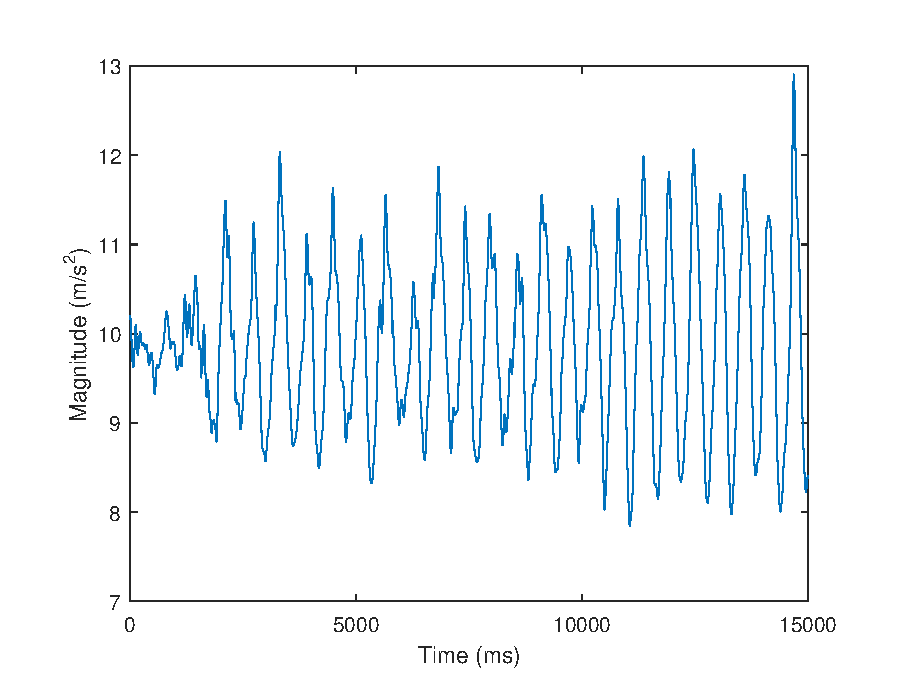
\includegraphics[width=\textwidth]{Images/accel_signal.eps}
            \centering
            \caption{Example of an accelerometer signal recorded during a period of walking.}
            \label{img_accel_ex}
        \end{figure}

        It is clear that each step will have both a peak and a trough associated with 2 and 4 respectively. The algorithm shall identify the peaks in the accelerometer signal. Effectively, the problem is one of peak detection in a noisy signal. 

        The algorithm is split into five stages, each responsible for a particular function. The data flows from stage to stage. All stages have an input data stream and output data stream, with the exception of the final stage which only has an input data stream. A block diagram is shown below in Figure \ref{img_sc_block}. Each one of the five stages will be described in detail in the following section.

        \begin{figure}[h]
            \includegraphics[width=\textwidth]{Images/step_counter_block.png}
            \centering
            \caption{Block diagram of the step counter algorithm.}
            \label{img_sc_block}
        \end{figure}

    \chapter{Algorithm Description}

        \section{Pre-Processing Stage}

            The Pre-Processing Stage is responsible for two functions:

            \begin{enumerate}
                \item Formatting the data received from the accelerometer into a usable format.
                \item Ensuring a constant sampling frequency by means of linear interpolation.
            \end{enumerate}

            The accelerometer data is received in the tri-axial format, however the algorithm is concerned with the magnitude rather than any single directional component because the the physical orientation of the device is unknown. The time stamps of the samples should also be scaled appropriately so that the first sample received from the user initiating the algorithm is at $t = 0$. The time stamps of the samples are provided in nanoseconds and are not given in standard UTC format, but as the time since system boot. The equations for these operations are simple and are as follows:

            \begin{equation}
                m = \sqrt{a_{x}^2 + a_{y}^2 + a_{z}^2},
            \end{equation}

            \begin{equation}
                t_{i,adjusted} = \frac{t_i - t_0}{t_s},
            \end{equation}

            where $m$ is the magnitude of the acceleration signal, $a_{x}$ is the acceleration in the x direction, $a_{y}$ is the acceleration in the y direction, $a_{z}$ is the acceleration in the z direction, $t_{i,adjusted}$ is the adjusted time stamp for the i-th sample, $t_i$ is the time stamp for the i-th sample, $t_0$ is the first time stamp in the trace, and $t_s$ is the time-scaling factor. For example, converting from nanoseconds to milliseconds, $t_s = 10^6$. 

            The data is then inserted into a simple data structure and is appended to an internal buffer of size 2. When this buffer is full, we will interpolate between these two points. The reason interpolation is needed is that although the developer can specific a desired sample rate in the Android application, there is no guarantee that the accelerometer will be sampled at this rate. An example of this is shown below in Figure \ref{img_sampling_freq} where time between samples is plotted against samples. For the filtering stage, we need to ensure that the data is sampled at a constant rate.

            The algorithm knows what the desired sample rate is, and will interpolate at this value. For example, if the sample rate is set to $f = 100 Hz$, then the algorithm will interpolate around $t = 0, 10, 20, 30, ... ms$. Each interpolated point is appended to the end of the stage's output data stream. The pseudocode for the linear interpolation is shown below.

            The equation for linear interpolation is as follows:

            \begin{equation}
                value = \frac{y_1 - y_0}{t_1 - t_0} t_{int} + y_0,
            \end{equation}

            where the two points that are being interpolated between are given by: $(t_1, y_1)$ and $(t_0, y_0)$, and the time to be interpolated at is given by $t_{int}$.

            \begin{figure}[h]
                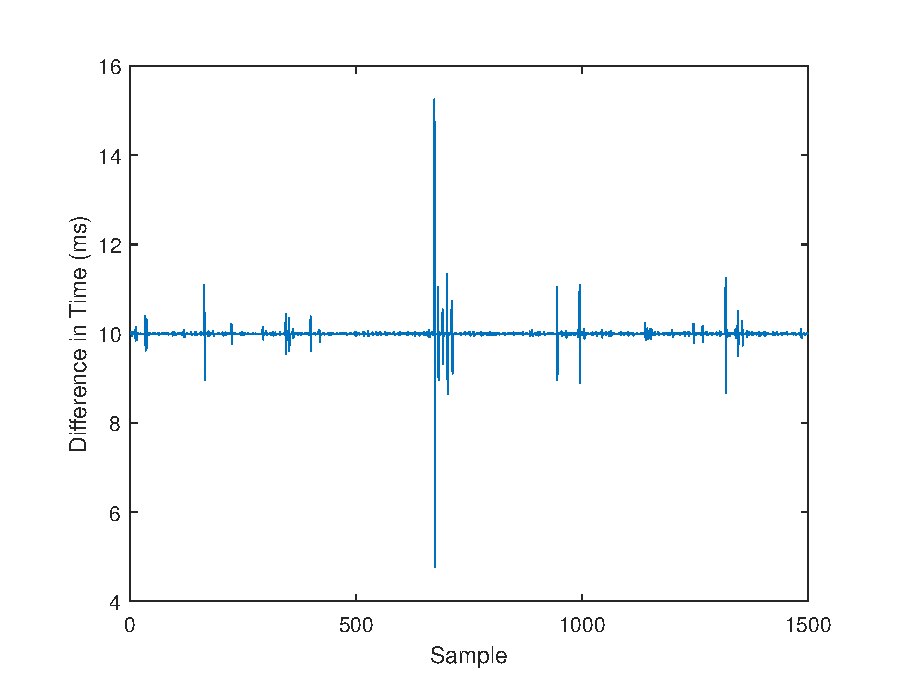
\includegraphics[width=\textwidth]{Images/sampling_freq.eps}
                \centering
                \caption{Time differences between samples for a 100Hz sampled signal. Note that the non-constant sampling times leads to the requirement for interpolation.}
                \label{img_sampling_freq}
            \end{figure}

        \section{Filtering Stage}

            The function of the filtering stage is to smooth the signal by removing as much of the high frequency noise from the acceleromater as possible.

            The filter required is a simple finite impulse response (FIR), low-pass digital filter. Ideally, this would be a steep-low pass filter with a frequency response described by Figure \ref{img_ideal_filter} below. However, this is impossible to achieve due to the infinite impulse response in the time domain (top-hat transforms to the sinc function). In order to capture the a variety of walking speeds, the cutoff of these filters will aim to be around 3 Hz. This should be sufficient to capture the walking of even the speediest walkers, as this would translate to an pace of $5.4 mph$ according to the ratio of $2000 steps = 1 mile$ as given by the American College of Sports Medicine [CIT]. Note that the average walking pace was found to be $3.1 mph$ in a study by Knoblauch, et. al. [CIT].



            A few filters were implemented for performance testing.

            \subsection{Moving Average}

                This is a very simple filter, each point in the filter window are weighted equally such that:

                \begin{equation}
                    m_k = \frac{1}{N},
                \end{equation}

                where $m_k$ is the $k^{th}$ filter coefficient, and $N$ is the length of the filter. The frequency response of this filter is shown below in Figure \ref{img_cm_filter}.

                \begin{figure}[!th]
                    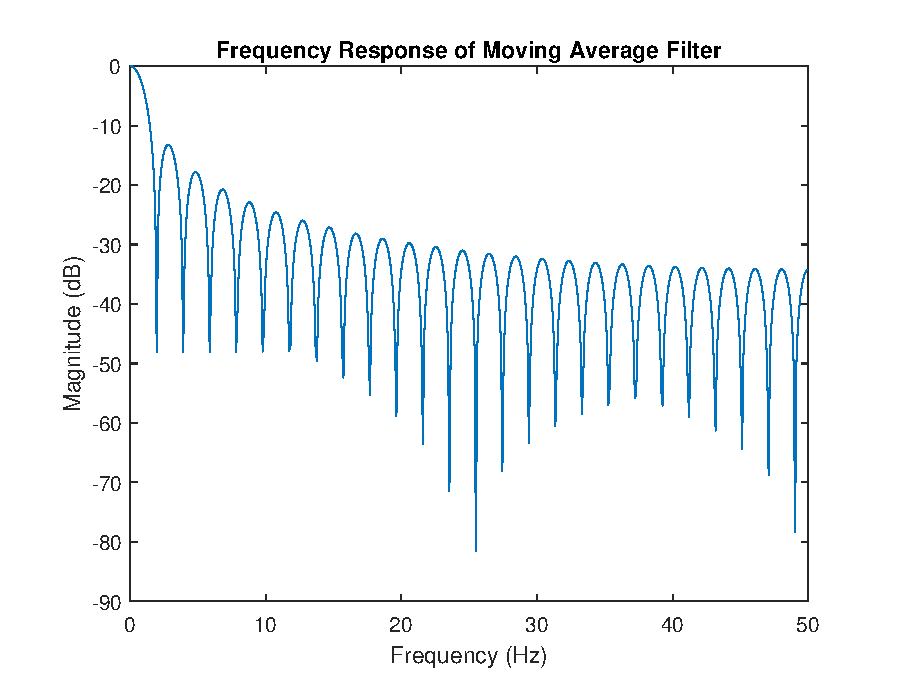
\includegraphics[width=\textwidth]{Images/cm_filter.eps}
                    \centering
                    \caption{Frequency response of the moving average filter with $N=31$.}
                    \label{img_cm_filter}
                \end{figure}

            \subsection{Gaussian Filter}

                This is a more complex filter, using a Gaussian as the waveform for the filter coefficients. This filter attempts to suppress the sidelobes of the center moving average filter by having a smoother transition to 0 magnitude. The weights of the filter are given by:

                \begin{equation}
                    g_k = \exp(-\frac{1}{2}(\frac{k - \frac{N-1}{2}}{\sigma \frac{N-1}{2}})^2),
                \end{equation}

                where $g_k$ is the $k^{th}$ coefficient of the filter, $N$ is the length of the filter window, and $\sigma$ is a parameter defining the standard deviation of the Gaussian. Note that the standard deviation also scales with the length of the filter. The frequency response of this filter is shown below in Figure \ref{img_ga_filter}.

                \begin{figure}[!th]
                    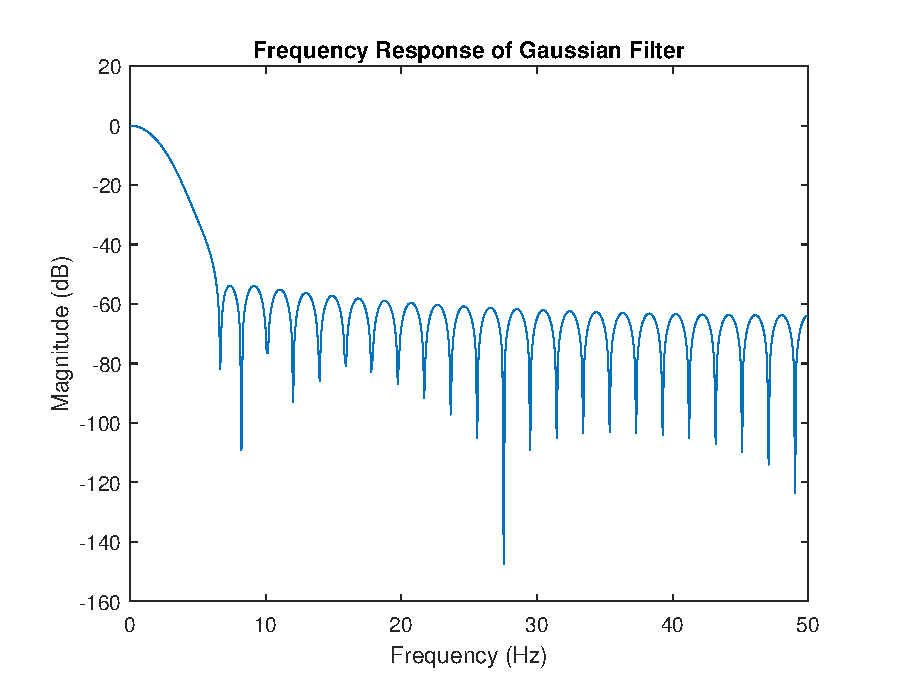
\includegraphics[width=\textwidth]{Images/ga_filter.eps}
                    \centering
                    \caption{Frequency response of the Gaussian filter with $N=51$ and $\sigma = 0.35$.}
                    \label{img_ga_filter}
                \end{figure}

            \subsection{Hann Filter}

                This is a similar filter to that of the Gaussian, where it attempts to smooth out the response by suppressing the sidelobes of the center moving average filter. The weights of the filter are derived from the Hann window [CIT] and are as follows: 

                \begin{equation}
                    h_k = \frac{1}{2}(1 - \cos(\frac{2\pi k}{N - 1}))
                \end{equation}

                where $h_k$ is the $k^{th}$ filter coefficient and $N$ is the length of the filter window. The frequency response of this filter is shown below in Figure \ref{img_ha_filter}.

                \begin{figure}[!th]
                    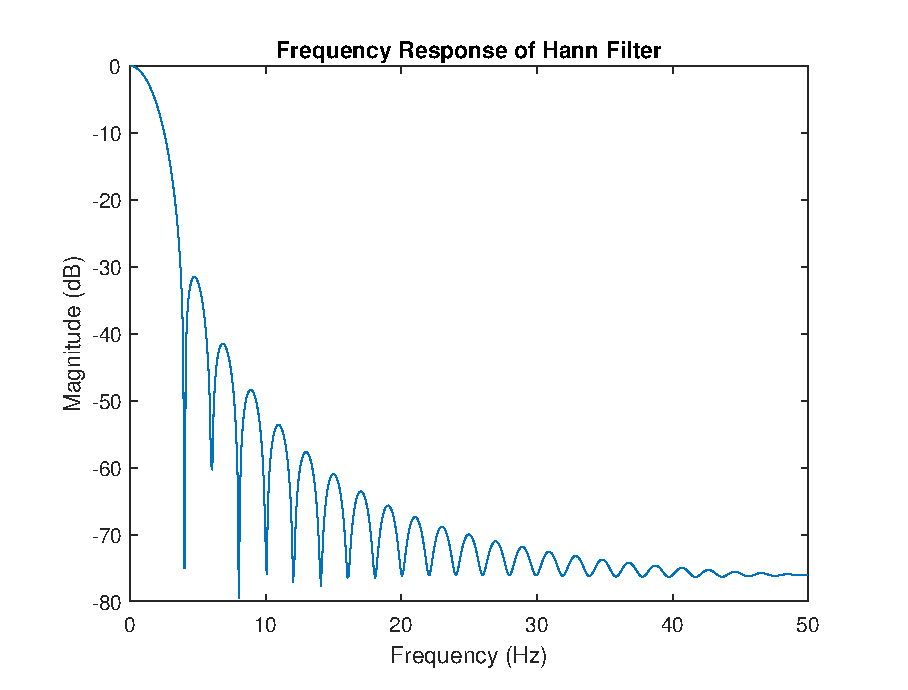
\includegraphics[width=\textwidth]{Images/ha_filter.eps}
                    \centering
                    \caption{Frequency response of the Hann filter with $N=51$.}
                    \label{img_ha_filter}
                \end{figure}  

            \subsection{Kaiser-Bessel Filter}

                This is the most complex filter design, designed by Kaiser [CIT] in order to achieve the desired attenutation at the cutoff frequency. It combines the ideal filter response (note a sinc function in the time domain) and a Bessel window to achieve the result. The calculation of the coeffcients are as follows.

                First, calculate the window shape parameter $\alpha$. 

                \begin{equation}
                    \alpha = 
                        \begin{cases}
                            0.1102(A - 8.7) & A \ge 50 \\
                            0.5842(A-21)^{0.4} + 0.07886(A-21) & 21 \leq A \geq 50 \\
                            0 & A \le 21
                        \end{cases},
                \end{equation}

                where $A$ is the desired attenuation at the cutoff frequency.

                Then calculate the coefficients of the Kaiser-Bessel window:

                \begin{equation}
                w_k = \frac{I_0(\alpha \sqrt{1 - (\frac{k - N_p}{N_p})^2})}{I_0(\alpha)},
                \end{equation}

                where $w_k$ is the $k^{th}$ coefficient of the window, $\alpha$ is the window shape parameter, $N_p$ is the midpoint of the filter, $N_p = \frac{N-1}{2}$ where $N$ is the length of the filter, and $I_0$ is the $0^{th}$ order Bessel function of the first kind.

                Then calculate the coefficients of the ideal filter response:

                \begin{equation}
                i_k = \frac{\sin(2\pi k\frac{F_c}{F_s})}{\pi k},
                \end{equation}

                where $i_k$ is the $k^{th}$ coefficient of the ideal filter response, $F_c$ is the desired cutoff frequency and $F_s$ is the sampling frequency.

                Finally, compute the coefficients of the filter with: 

                \begin{equation}
                b_k = w_ki_k,
                \end{equation}

                where $b_k$ is the $k^{th}$ coefficient of the Kaiser-Bessel filter response. The frequency response of this filter is shown below in Figure \ref{img_kb_filter}.

                \begin{figure}[!th]
                    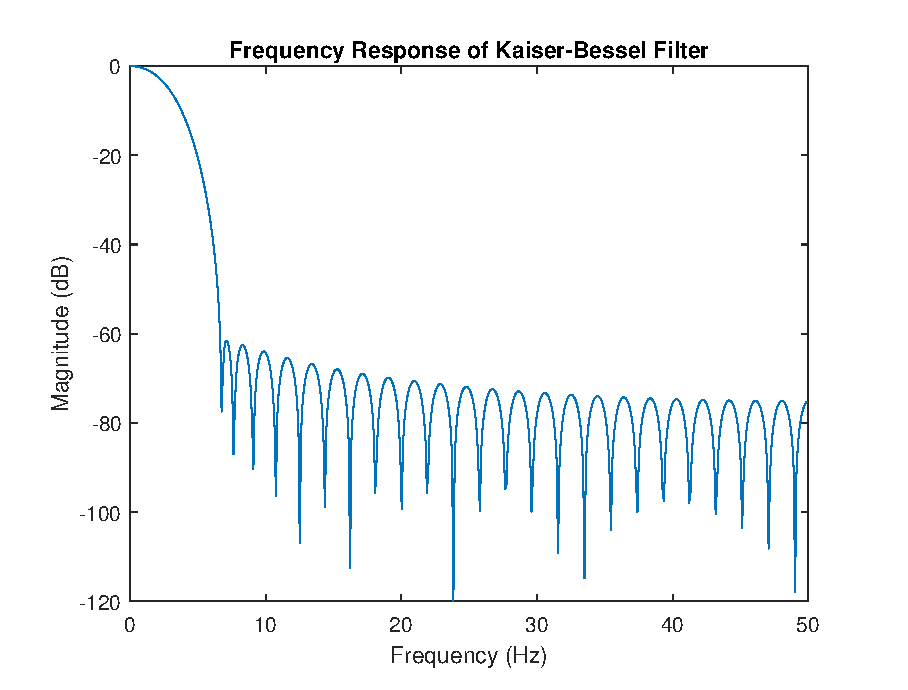
\includegraphics[width=\textwidth]{Images/kb_filter.eps}
                    \centering
                    \caption{Frequency response of the Kaiser-Bessel filter with $N=51$, $A=60dB$, $F_c = 3Hz$, and $F_s= 100Hz$.}
                    \label{img_kb_filter}
                \end{figure}  

        \section{Scoring Stage}

        \section{Detection Stage}

        \section{Post-Processing Stage}

    \chapter{Data Collection Apparatus}

    \chapter{Algorithm Optimization}

    \chapter{Results}

    \chapter{Further Work}
\part{Sleep Detection}

    \chapter{Overview}

        This section covers the development and evaluation of the sleep detection algorithm. The algorithm aims to extract features like sleep onset time, wakefulness onset time, and total time asleep from accelerometer data recorded on a wrist-mounted device.

        The basis of this algorithm relies on the fact that the level of activity of a person can be determined from the magnitude of the standard deviation or the energy of the accelerometer signal. If there is no movement, the standard deviation should be the square root of the variance of the noise in the accelerometer sensor (assumed to be zero-mean Gaussian). If there is a high level of movement, then there will be a high standard deviation from the signal. If there is a long period of low activity then this period will be defined as asleep. This set of rules and inferences will be the guiding principles upon which the algorithm is built.

        All of the data used in the algorithm development and validation was analysed at 10Hz.


    \chapter{Database}
        \label{c-database}

        The algorithm development and testing the following chapter relies heavily on a database created by Borazio, et. al. at TU Darmstadt [CIT]. The database contains accelerometer data from 42 patients, their clinically annotated polysomnography results, and light sensor data from overnight stays in a sleep lab. The accelerometer data comes from a custom device that is mounted on the wrist of the patient. The data is logged at 100Hz. 

        The data provided is contained and compressed in such a way that requires reformatting for the use described below. Each patient record has its own file (a .npy file, used for Numpy calculations in Python) which contains 7 columns: a timestamp, the runlength encoding, x-acceleration, y-acceleration, z-acceleration, light sensor value, and a ground truth value. The runlength encoding represents how many times in a row does the following set of measurements repeat, for example runlength encoding of $10$ represents 10 sequential copies of this row with increasing timestamps. All of the acceleration data is stored in an 8-bit unsigned int, from 0 to 255. According to Borazio, et. al. this should map to $-4g$ to $4g$, where $g$ is gravity. The light sensor value is not used in this project and as such will be disregarded. The ground truth is marked as follows: 0 indicates unknown sleep state, 1-3 maps to different sleep states rated from deepest to lightest, 5 indicates random eye movement (REM) sleep, 6 indicates awake, and 7 indicates movement.

        In order to format this data better to the needs of this project a few steps were taken:

        \begin{itemize}
            \item The x,y, and z accelerations will be linearly mapped back to $[-4g,4g]$ and the magnitude will be taken.
            \item The light sensor value will be stripped from the data.
            \item The runlength encoding will be decoded and this column shall be redundent and thus removed.
            \item The data will be downsampled to $10Hz$ to conform with the project specifications.
        \end{itemize}

        The downsampling is a simple operation: keep one point out of every 10 after the runtime encoding decoding is complete. Decoding the runlength encoding is equally simple: duplicate the row of $n$ times where $n$ is the runlength encoding for that row.

        \section{Remapping of Acceleration}

            This operation is fairly straightforward: an original value of $127.5$ is remapped to $0g$ and thusly the value of acceleration can be derived from:

            \begin{equation}
                a_n = (a_o - 127.5)*\frac{8*g}{256}
            \end{equation}
            where $a_n$ is the new acceleration value, $a_o$ is the old value of acceleration, and $g=9.81\frac{m}{s^2}$ is gravity. The format that the acceleration was stored in limits the resolution of the each component, but the combination of the components to the magnitude increases the magnitude slightly.

            This approach is validated by ensuring that the magnitude of the signal is gravity or higher, this is true for the dataset hence this approach is appropriate.



    \chapter{Algorithm Description}

        The algorithm works in two stages: the prediction stage and the post-prediction filter.

        \section{Pre-Prediction Filter}

            Originally, the design included a pre-prediction filter, however this was removed as it degraded overall performance. The implementation and explanations for its removal will be explained here.

            This was aimed to take the accelerometer data and remove high frequency noise and spikes from the signal. This is done through a simple moving average filter.

            Hence, the coefficients of the filter are as follows:

            \begin{equation}
                h_k = \frac{1}{N}, 1\leq k\leq N
            \end{equation}
            where $h_k$ is the $k^{th}$ coefficient of the filter and $N$ is the length of the filter.

            The frequency response of this filter can be seen below in Figure \ref{img_pp_filter}. Body movements are generally slow, so the filter effectively removing higher frequency data is permissible in this use case.

            \begin{figure}[h]
                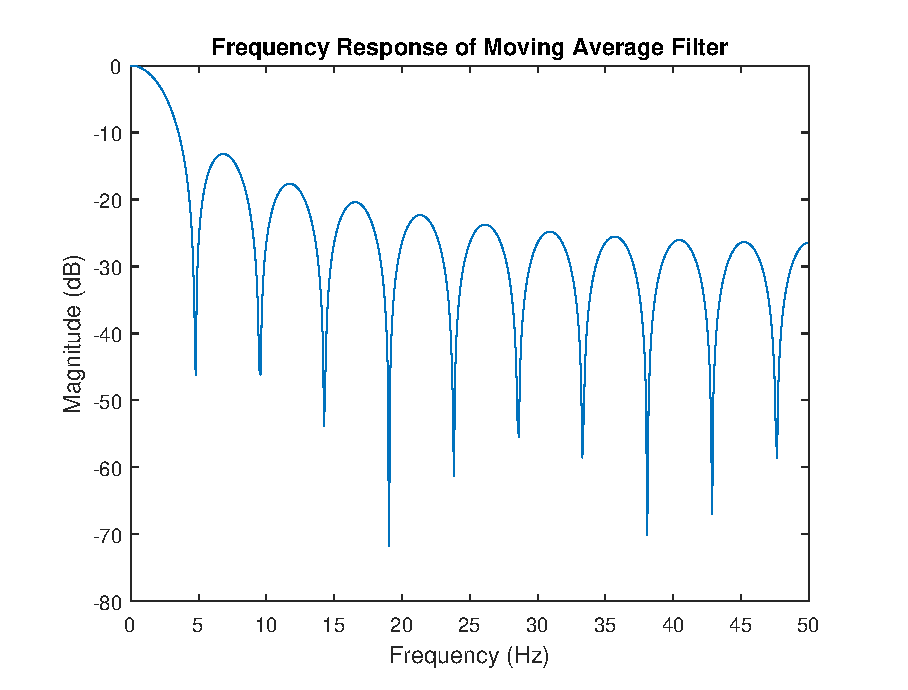
\includegraphics[width=\textwidth]{Images/sleep_pre_filter.eps}
                \centering
                \caption{Frequency response of the pre-prediction filter with a length of 21 samples.}
                \label{img_pp_filter}
            \end{figure}

            An example of the data before filtering and after filtering can be seen below in Figure \ref{img_pp_filter_ex}.

            \begin{figure}[h]
                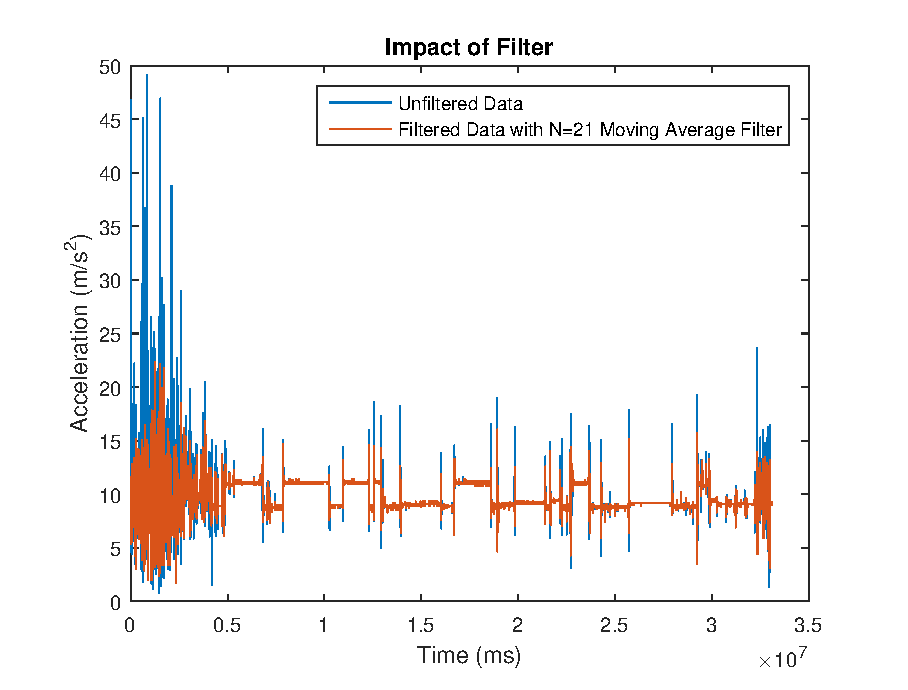
\includegraphics[width=\textwidth]{Images/sleep_pre_filter_ex.eps}
                \centering
                \caption{Example of data before and after filtering. Blue is before filter, orange is after filter. Note the reduced magnitude in the active areas (areas of high magnitude.)}
                \label{img_pp_filter_ex}
            \end{figure}

            However, this graph illustrates why the filter had to be removed. It suppresses areas of high activity thus reducing the standard deviation. This is a direct impact on the quantity that we wish to measure and thus is degrading the information content. Removing the filter increased the algorithm accuracy by around 5\%.           

        \section{Prediction Stage}

            The next stage of the algorithm is to predict whether a chunk of the signal is asleep or awake. The signal is segmented into chunks of 600 samples long, this is equivalent to a period of 1 minute at a 10Hz sampling frequency. This period was chosen as it is close to what one might consider the characteristic length of being asleep. For example, it seems absurd to consider wakefulness on a second by second basis. It also allows for enough information to be captured in the chunk to allow meaningful analysis.

            The prediction is done through a logistic regression, the coefficients of which have been obtained through an optimization process described below in Section \ref{ss_coefficients}.

            The logistic predictor is defined as:

            \begin{equation}
                p(\mathbf{x}, \mathbf{m}) = \frac{1}{1 + e^{-\mathbf{mx}}}
            \end{equation}
            where $\mathbf{x}$ is the feature vector and $\mathbf{m}$ is the coefficient vector. If $p(\mathbf{x}) \geq 0.5$ then that point is classified as asleep (or 1). Otherwise is is classified as awake (or 0).

            \subsection{Coefficients}
                \label{ss_coefficients}

                The feature vector selected for prediction is simple and contains 2 elements: a constant, and the standard deviation. This is defined as follows: 

                \begin{equation}
                    \mathbf{x} = \begin{bmatrix} 1 & \sigma \end{bmatrix}
                \end{equation}

                In order to learn the coefficients, each data segment must have a known ground truth value. That is to say, it is known if the person was awake or asleep during that segment. The database described above was used in acquiring this necessary data. The data was formatted and downsampled like described above in Section \ref{c-database} and then filtered through the moving average filter in the preceeding section. Each data recording was then scanned to look for contiguous periods of sleep or wakefulness. These periods had to be 600 samples long and represented the extremes for a data segment where all of the segment is classified as awake or asleep. These periods were extracted and the feature vector for each was pre-calculated. This dataset would serve as the training and test data for learning the coefficients. 

                In order to optimize the data, a loss function is needed to minimize. This function should encapsulate penalties for incorrect results. 

                To derive this, start with the likelihood of the coefficients given the data:

                \begin{equation}
                    \mathcal{L}(\mathbf{m}) = \prod_{i=1}^n p(y_i|\mathbf{x_i}, \mathbf{m})
                \end{equation}
                where $\mathcal{L}(m)$ is the likelihood of the coefficients, $y_i$ is the ground truth of the $i^th$ data point.

                If the log-likelihood is considered, then this expression can be expanded to:

                \begin{equation}
                    \log{\mathcal{L}(\mathbf{m})} = \sum_{i=1}^n (y_i\log{p(\mathbf{x_i}, \mathbf{m})} + (1-y_i)\log{(1 - p(\mathbf{x_i}, \mathbf{m}))})
                \end{equation}
                where the first term under the summation represents the contribution to the likelihood when $y_i = 1$ and the second term represents the contribution when $y_i = 0$.

                If the log-likelihood is differentiated with respect to $\mathbf{m}$ then it can be shown that the differential is given by:

                \begin{equation}
                    \frac{\partial}{\partial \mathbf{m}}\log{\mathcal{L}(\mathbf{m})} = \sum_{i=1}^n (y_ip(\mathbf{x_i}, \mathbf{m})\mathbf{x_i} - (1-y_i)(1 -p(\mathbf{x_i},\mathbf{m}))\mathbf{x_i})
                \end{equation}

                Unfortunately, this expression has no closed form solution if set to zero (i.e. - if optimizing). In light of this, the logistic regression can only be optimized from methods like gradient descent. The premise of gradient descent is simple, calculate the gradient at a point and then move either up or down the gradient, for maximization and minimization respectively. The downside of this method is that there is no guarantee of getting the global maximum, merely the local maximum. 

                In this project, gradient descent was performed with 200 iterations and a learning rate of $\nu = 0.00004$. Half of the data was used for training and the other half was used for testing. After validating the consistency of the results, the coefficients yielded are given by:

                \begin{equation}
                    \mathbf{m} = \begin{bmatrix} 0.5707 & -2.6377 \end{bmatrix}
                \end{equation}
                where the first coefficient is related to the constant and the second coefficient is related to the standard deviation. The training data had a final accuracy with these coefficients of 72.9\% and the testing data had an accuracy of 71.2\% which shows the data was not overfitted to the training data.

                In fact, since there is only one variable in the regression, the regression acts much like a decision boundary. This can be plotted out quite easily as seen in Figure \ref{img_regression}.

                \begin{figure}[h]
                    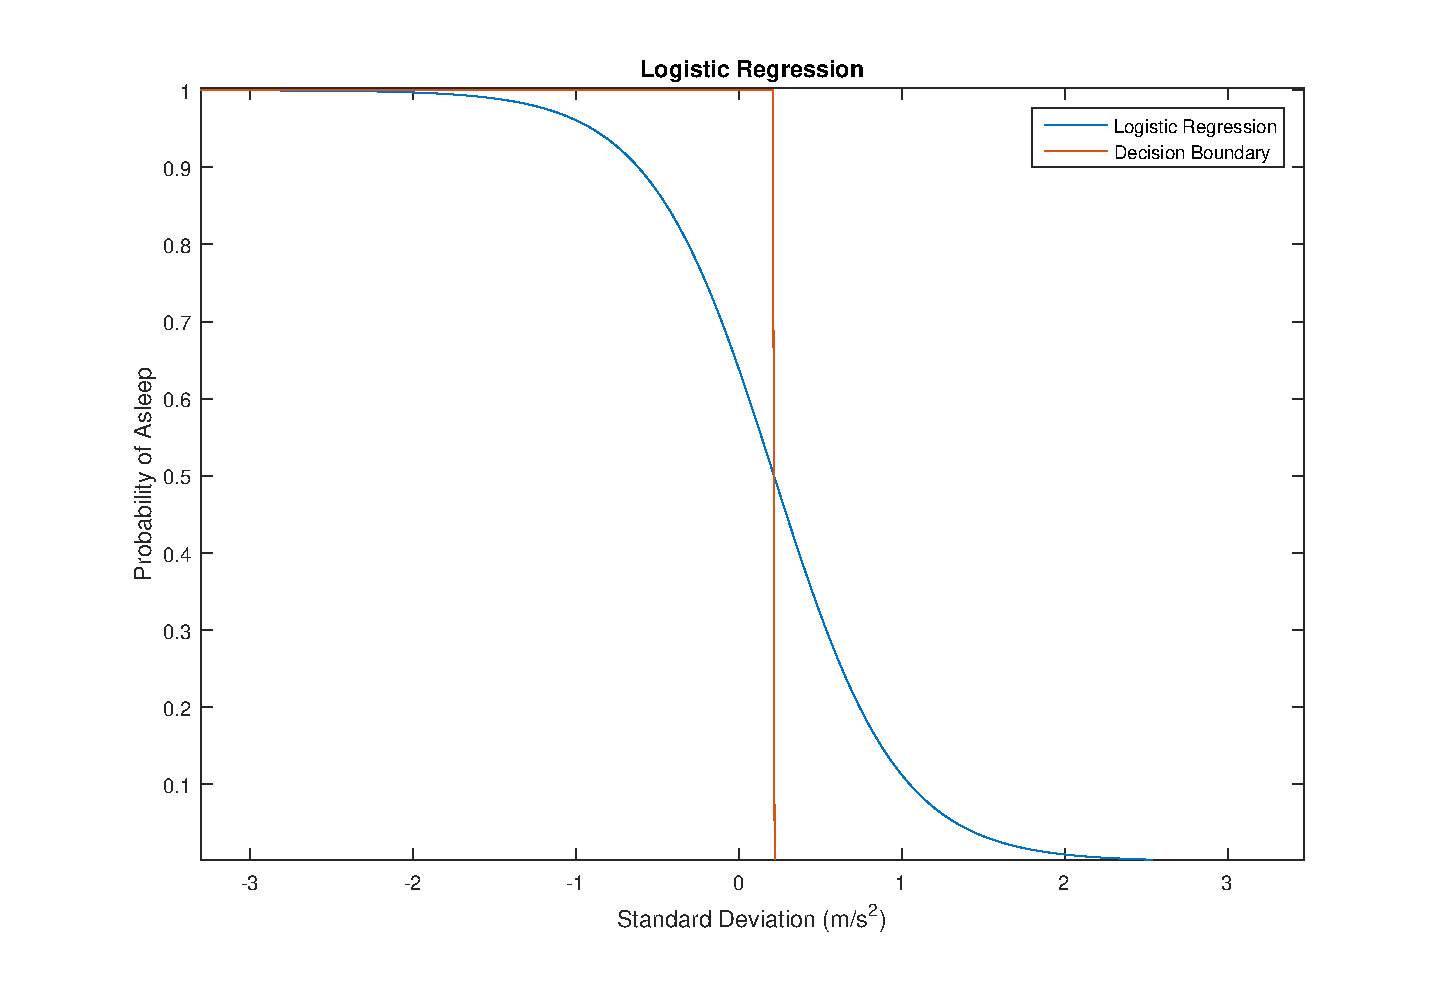
\includegraphics[width=0.75\textwidth]{Images/logistic_regression.eps}
                    \centering
                    \caption{A plot of the standard deviation of a signal segment against the probability of asleep. The step function represents the simplified decision boundary due to the single variable used.}
                    \label{img_regression}
                \end{figure}

                An example of the data under prediction can be seen below in Figure \ref{img_regression_ex}.

                \begin{figure}[h]
                    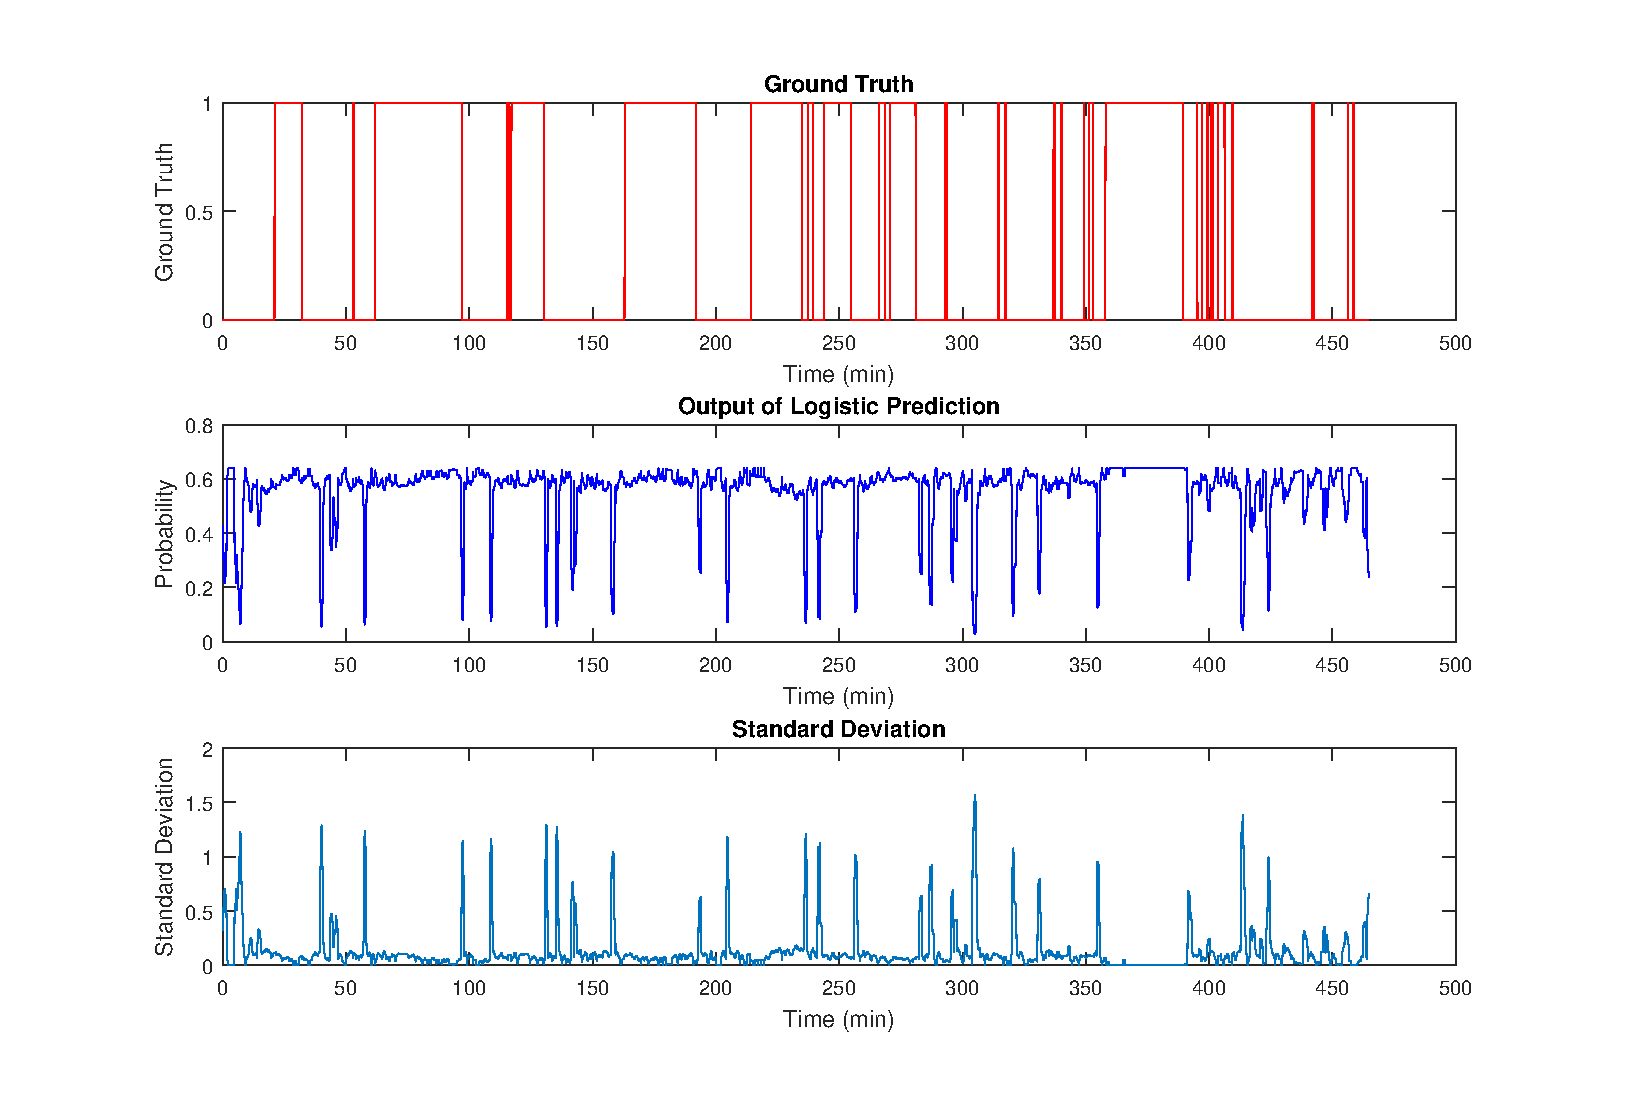
\includegraphics[width=0.8\textwidth]{Images/logistic_regression_ex.eps}
                    \centering
                    \caption{This is an example of the logistic regression making predictions based on standard deviation. Note how as standard deviation increase, the probability output decreases.}
                    \label{img_regression_ex}
                \end{figure}

        \section{Post-Prediction Filter}

            The next and final stage is a post-prediction filter. This stage exists due to the fact that classifying sleep for $100$ms periods is absurd for a detector based on an accelerometer signal. It is reasonable to assume that for our purposes, the minimum sleep time detectable is roughly $5$ minutes. This leads to the filter length discussed later on.

            The implementation of this filter works as a threshold, that is to say, if the output of the filter is above some value, the value gets rounded up and all other values get rounded down. This is to maintain the 0-1 classification inherent in the problem. 

            A window is taken around the point in question and the filter looks $k$ points to the left and $k$ points to the right of this point and the filter value is calculated by:

            \begin{equation}
                f_n = \sum_{i=-k}^k h_ix_{n+i}
            \end{equation}
            where $f_n$ is the filter value at the $n^{th}$ point, $h_i$ is the $i^{th}$ filter coefficient and $x_{n+i}$ is the $(x+i)_{th}$ point. If $f_n$ exceeds $t$, a chosen threshold, then the $n^{th}$ point is marked as asleep. $k$ is set to $1500$ for this filter, deriving from the $5$ minute minimum. 

            Two windows were considered for this filter: a moving average window (flat) and a Gaussian window. Each of these represents a different approach to the filter. The moving average window indicates that each point inside the window is valued equally, that is to say, the point $k$ timesteps away from the point under consideration is weighted the same as the point under consideration. The Gaussian windows is the opposite of this, points closer to the point under consideration are weighted more heavily than those farther away.

            A small script was written to select the best performing filter parameters: the threshold, $t$ would be varied for both filters from $0.85$ to $0.975$ at $0.025$ increments and the standard deviation, $\sigma$, for the Gaussian filter would be varied from $1000$ to $3500$ at $250$ increments. The threshold values were chosen in keeping with the idea that sleep will be fairly continuous along a signal, that is to say, the majority of datapoints should be positively classed as asleep in order to mark an area as asleep. The $\sigma$ values were chosen to align with the filter length of $3001$, this ensures that all values get a non-negligible weight, as filter coefficients at points outside of the $\begin{bmatrix}-2\sigma & 2\sigma \end{bmatrix}$ range are effectively given zero weighting.

            The best performing filter was the Gaussian with $t=0.975$ and $\sigma=2000$. An example of this post-prediction filter in action is shown below in Figure \ref{img_post_filter_ex}.

            \begin{figure}[h]
                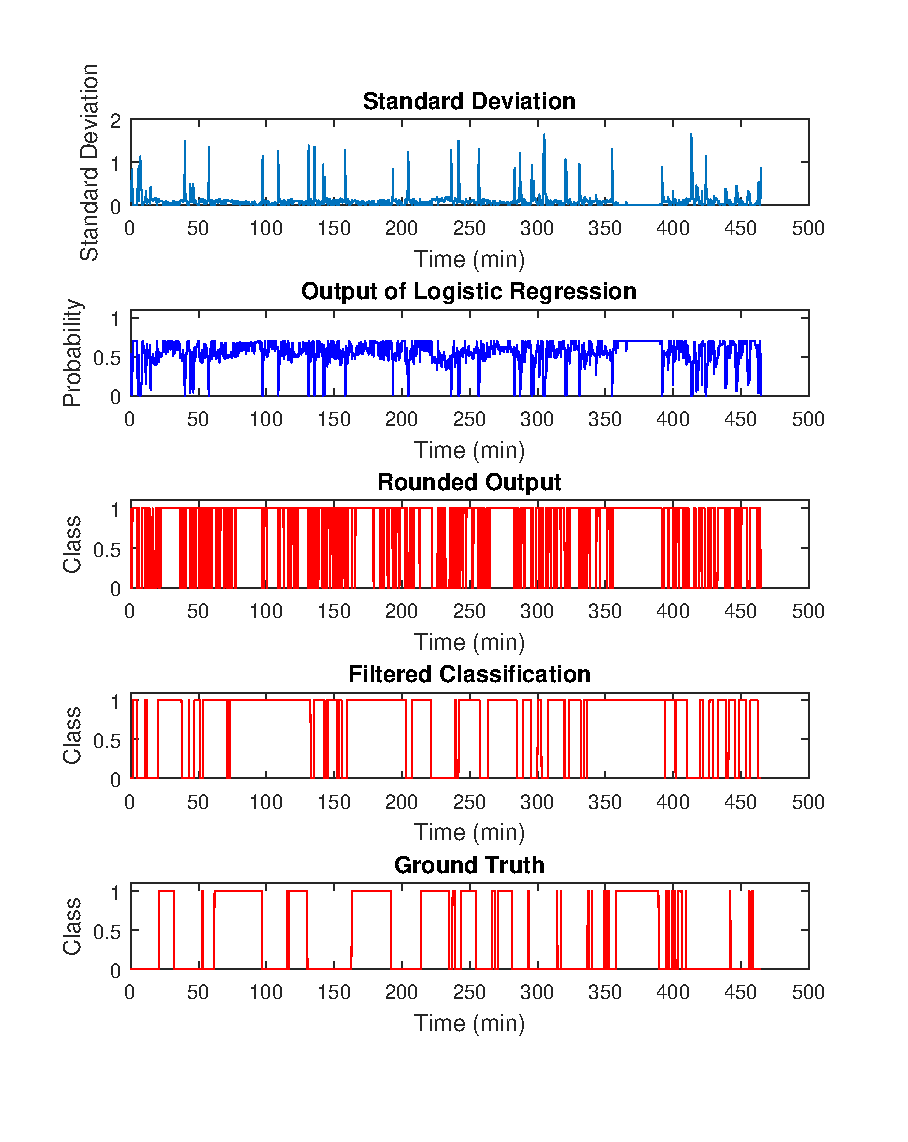
\includegraphics[width=0.8\textwidth]{Images/post_prediction_filters_ex.eps}
                \centering
                \caption{An example of the predicted output being filtered. The filter used was a Gaussian filter with length 3001 and standard deviation of 2000.}
                \label{img_post_filter_ex}
            \end{figure}


    \chapter{Results}

        The results presented here are a result of running the algorithm as described above, with no pre-prediction filter over $45$ of the $46$ data records in the Darmstadt database. One of the records was rejected as there was very little sleep in the record and the data was inconsistent throughout.

        An example of the algorithm classification in action can be seen in Figure \ref{img_ex_data_recording}. Note that a state of 1 indicates sleep, a state of 0 indicates wakefulness. 

        \begin{figure}[h]
            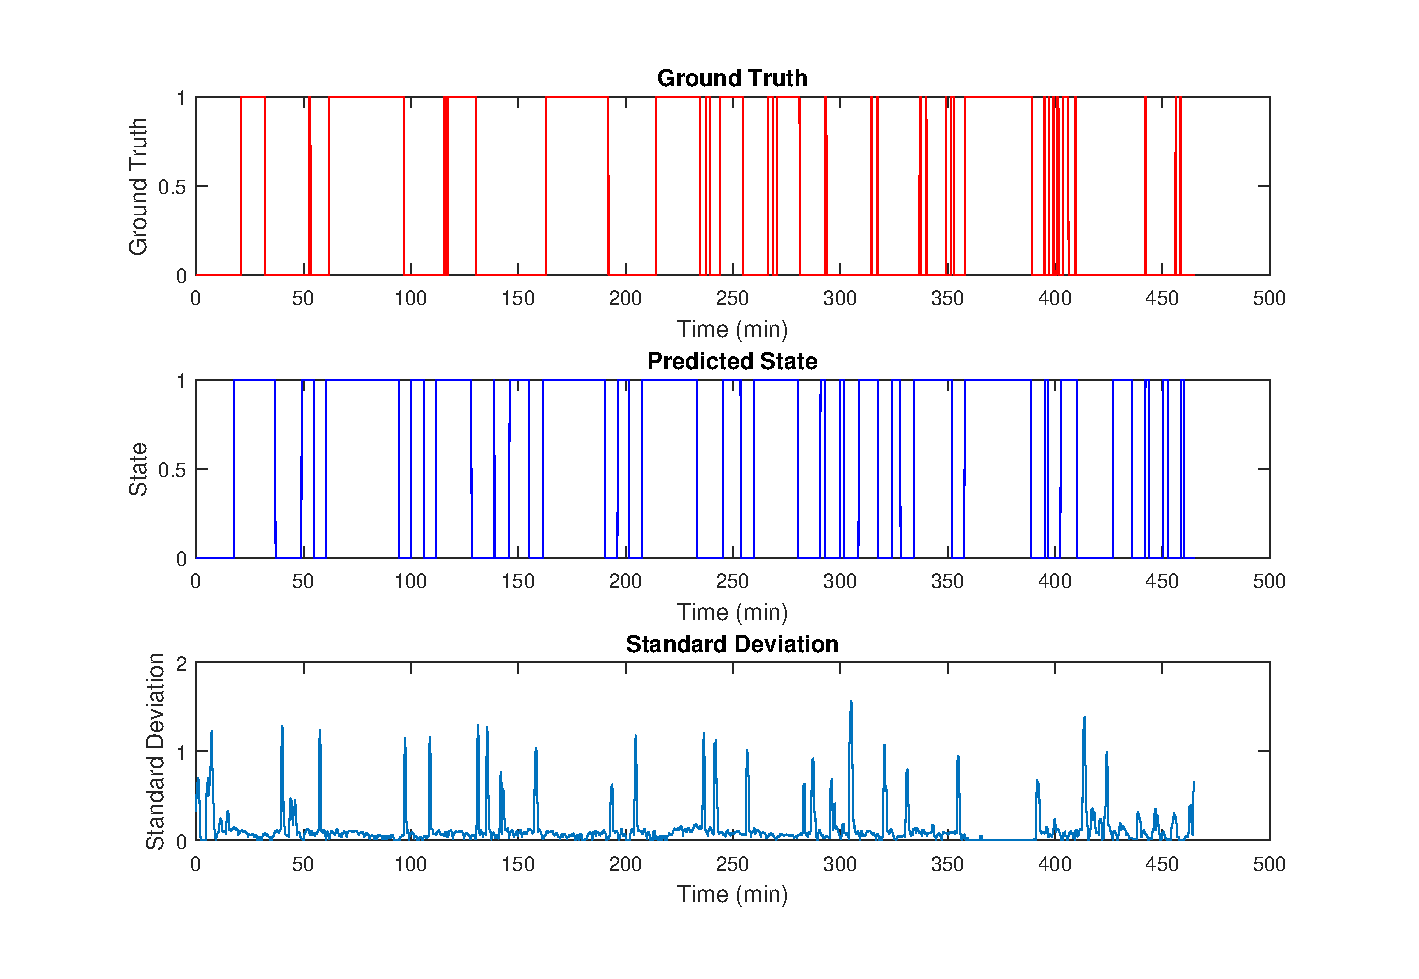
\includegraphics[width=\textwidth]{Images/example_data_recording.eps}
            \centering
            \caption{Example of the classification algorithm. From top to bottom: ground truth, predicted state, standard deviation.}
            \label{img_ex_data_recording}
        \end{figure}

        \section{Statistics}

            The algorithm is judged on 3 metrics: the Total Time Asleep (TTA), the total amount of sleeping time in the record, the Sleep Onset Time (SOT), the timestamp of the first incidence of sleep, and the Wakefulness Onset Time (WOT), the timestamp of the last incidence of sleep. The latter two parameters are representative of the start and end of a night's sleep. 

            For the algorithm described above, the following errors are achieved.

            \begin{center}
                \captionof{table}{Errors for the sleep detection algorithm.}
                \label{tbl_sleep_errors}
                \begin{tabular}{|c||c|c|}
                    \hline
                    Metric & Mean Error & Median Error \\
                    \hline
                    Total Time Asleep (\%) & 21.74\% & 11.89\% \\
                    Sleep Onset Time (minutes) & 25.08 min & 19.75 min \\
                    Wakefulness Onset Time (minutes) & 13.35 min & 3.86 min \\
                    \hline
                \end{tabular}
            \end{center}

            This performs better than the algorithm described in Borazio, et. al. [REF] that achieved 21.17\% median error for Total Time Asleep. This is almost a 10\% increase. The paper from Borazio, et. al. makes no mention of SOT or WOT statistics, so there can not be a comparison here.

            From the results, it is clear that all the error statistics have outliers far from the median since $e_{mean} > e_{median}$ for all the statistics. This is confirmed by the boxplots of the errors in Figures \ref{img_tta_error} and \ref{img_sot_wot_error}. For example, in the boxplot of TTA there are a number of outliers that skew the mean away from the median, but the bulk of the errors reside in between $0\%$ and $32\%$ error. 

            \begin{figure}[h]
                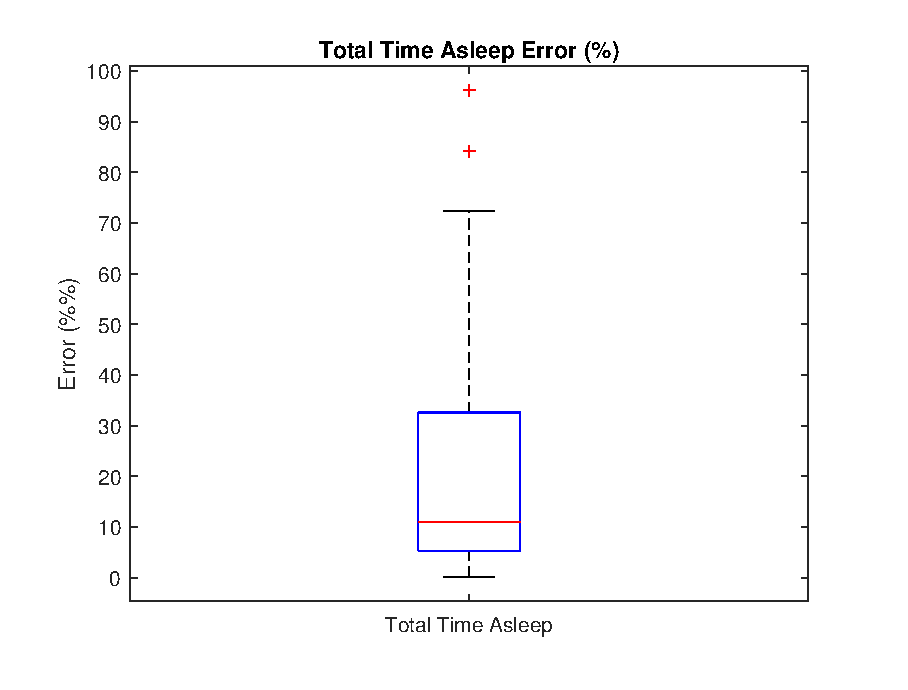
\includegraphics[width=0.75\textwidth]{Images/tta_error.eps}
                \centering
                \caption{Boxplot of errors for the Total Time Asleep. Median is at 11.89\%.}
                \label{img_tta_error}
            \end{figure}

            \begin{figure}[h]
                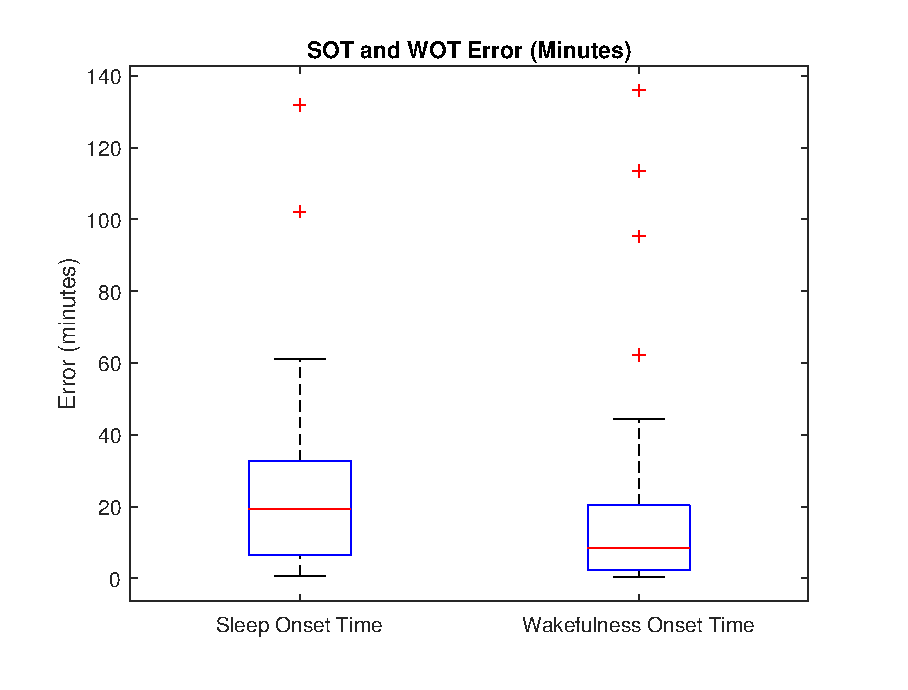
\includegraphics[width=0.75\textwidth]{Images/sot_wot_error.eps}
                \centering
                \caption{Boxplots of errors for the Sleep Onset Time and Wakefulness Onset Time. Note that the WOT is generally more accurate than the SOT.}
                \label{img_sot_wot_error}
            \end{figure}

            Another interesting thing is to examine the difference in accuracy between the SOT and WOT, as these fundamentally represent the two abilities of the algorithm: to identify sleep segments and to identify wakeful segments respectively. One explanation of the WOT being generally more accurate is that the end of sleep is generally very near to the end of the recording. So it could be a case of the recording ending limits the WOT error, whereas a similar phenomenom does not occur with the SOT.

        \section{Precision and Recall}

            A sensible way of quantifying these abilities is to look at the algorithm's precision and recall for both sleep states and awake states. Precision is defined as "the fraction of retrieved instances that are relevant" and recall is defined as "the fraction of relevant instances that are retrieved" [REF]. In this case, the sleep precision would be the percentage of predicted sleep states that are sleep states in the ground truth and the sleep recall would be the percentage of ground truth sleep states that were predicted sleep states. A similar description follows naturally for the wakeful states. The precision and recall were calculated on a per recording basis and tabulated for the entire algorithm. The results of this can be seen in Figure \ref{img_prec_recall}.

            \begin{figure}[h]
                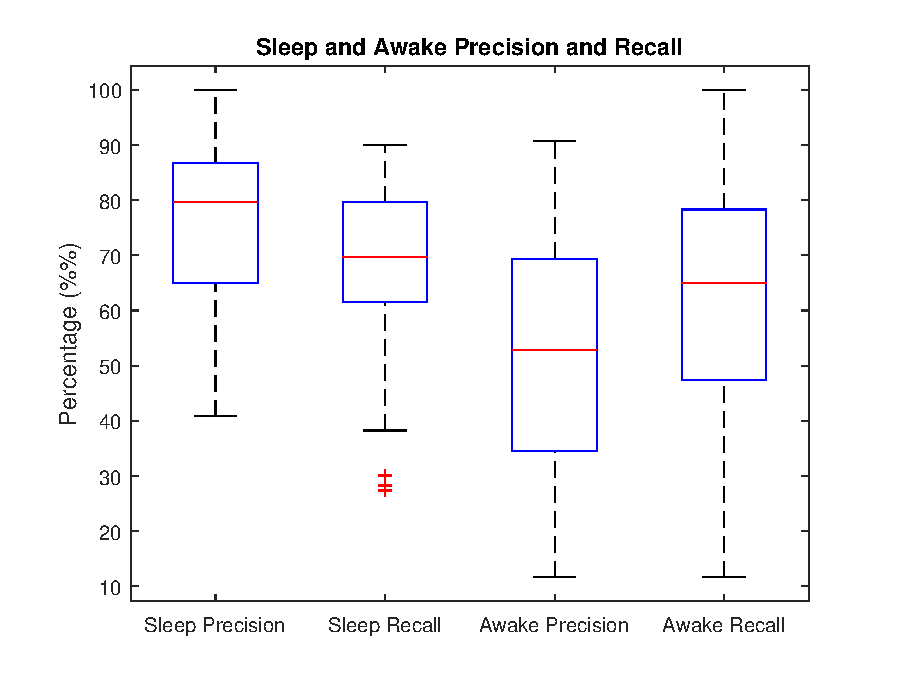
\includegraphics[width=0.75\textwidth]{Images/prec_recall.eps}
                \centering
                \caption{Boxplots of precision and recall for sleep and awake states. From left to right: sleep precision, sleep recall, awake precision, awake recall.}
                \label{img_prec_recall}
            \end{figure}

            The first thing to note is that the sleep precision is generally higher than that of awake. An explanation of this is that the algorithm is more biased toward classifying a point as awake than sleep. This means that the points that are classified as sleep are more likely to be sleep since the bar for classification is much for this. Another thing to note is that there is a very large variance in the awake precision and recall. This means that the algorithm generally had a hard time correctly identifying awake states. The awake recall being higher than precision indicates again that the algorithm tended to overclassify as awake. This is further supported by the recall of sleep being higher than the precision, also indicating that the algorithm is biased toward classifying as asleep. 

            This is interesting as in Borazio, et. al. the authors experienced the opposite case, along with the Cole [REF] and Oakley [REF] algorithms, in that they tended to overclassify as sleep. This is evidenced by the awake recall being much higher in this algorithm (65\% median vs. 45\% for Borazio, et. al.). This comes at the cost of a reduced sleep recall (70\% vs 94\% for Borazio, et. al.). Overall, this leads to a more balanced algorithm that is more equally adept at identifying sleep and awake states.


    \chapter{Further Work}

        Although small improvements were made to the sleep detector, there is still room for significant improvement. One area that can be explored is extending the feature vector used for prediction. Other features of the signal segment like the skewness or kurtosis of the distribution can be explored or examine the frequency content in the signal and attempt to correlate this with sleep states. Ultimately, this approach is limited due to the simple fact that it is impossible to discern the situation where someone is awake and not moving and the situation where someone is sleeping. One other area of interest is exploring extending the algorithm to include more sensors than the accelerometer like recording heartrate or the magnitude of light and using these factors as additional features. The structure of the algorithm is designed to accomodate additional features as these can simply be added to the feature vector without otherwise changing the algorithm.
\part{Conclusion}
\chapter{Conclusion}

This project set to do two main things: develop a general step counter implemented on a smartphone that uses an accelerometer as its data source and develop a sleep detection algorithm that uses a wrist mounted accelerometer as its data source. 

The generalized smartphone step counter exhibits very high accuracies with a median of 96.8\% across a variety of scenarios. A number of scenarios like: phone in pocket, phone in hand, etc. were examined and specific parameters for these scenarios were derived with even higher levels of accuracy than the general parameters. The general algorithm was further validated against three data recordings from patients which resulted in similar statistics showing that it is truly general. The step counter algorithm is also modular and can be subject to further improvement and optimization as it was developed modularly and has an infrastructure built around it to enable rapid iteration. 

The sleep detection algorithm was developed against an existing database and outperformed previous algorithm attempts on this database with 10\% error reduction in Total Asleep Time. Compared to previous attempts, which tended to overestimate sleep, this algorithm managed to be more balanced in its estimation which is a contributing factor to the higher accuracy. Similar to the step counting algorithm, the sleep detection algorithm is also built with iterations in mind, as minimal changes would be needed to introduce new features into the feature vector for classification. 

These two algorithms introduce new tools into the medical healthcare professional's toolkit that enable rapid and cheap data collection. This data can then be used to help inform medical decisions. The data collection can be done at home, without the presence of medical professionals or expensive equipment. The expanding proliferation of smartphones and smart devices mean that this sort of approach can become more widespread, reducing healthcare costs and increasing the data available to professionals. 
\printbibliography[title={References}]
\includepdf[pages={1}]{Text/risk_1.pdf}
\includepdf[pages={1}]{Text/risk_2.pdf}

\end{document}